\section{Valgrind}

\subsection{Outils de Valgrind}
\begin{itemize}
\item Memcheck : Détection d'erreur mémoire (accès à de la mémoire non-allouée, valeurs non initialisées, double free, memcpy, fuites) 
\item Cachegrind : Profiler de mémoire cache (hit et miss)
\item Callgrind : Profiler de cache avec infos supp et graph
\item Helgrind : Détection d'erreur de threads 1
\item DRD : Détection d'erreur de threads 2
\item Massif : Profiler de heap et stack (mémoire restante, leaks)
\item DHAT : Profiler de bloc dans le heap
\end{itemize}

\subsection{Utilisation des outils}
\begin{figure}[H]
    \centering
    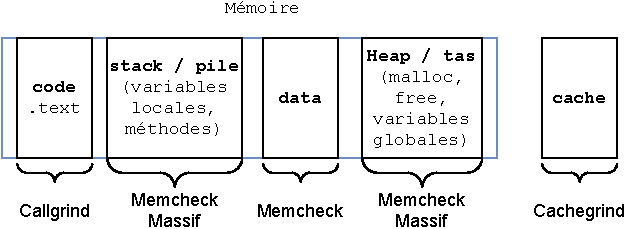
\includegraphics[width=0.6\columnwidth]{valgrind.pdf}
\end{figure}

\subsection{Trouver le bon outil}
L'outil Memcheck regroupe beaucoup de fonctionnalité. C'est lui qu'il faut utilisé en priorité
